The continuum body $\Omega$ is discretized into a set of $N_p$ material points in an arbitrary Cartesian grid made of  $N_n$ nodes and $E$ non-overlapping cells of volume $\Omega^e $ (a two-dimensional example is depicted in figure \ref{fig:domain}).
% The boundary of the domain is again defined by the set of edges separating empty cells from those containing particles (see figure \ref{fig:domain} for a two-dimensional example).
\begin{figure}[ht]
  \centering
  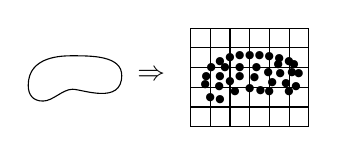
\begin{tikzpicture}[scale=0.25]
  % \draw[step=1.0,black,thin] (-3.,-1.) grid (3,4.);
  % \draw (-3,-1) -- (3,-1) -- (3,4) -- (-3,4) -- (-3,-1);
  \begin{scope}[scale=0.5]
    \draw (-3,0.6) .. controls +(1,0) and +(-1,0) .. (0,1.8)  
    .. controls +(1,0) and +(0,-3) .. (5,3.2) 
    .. controls +(0,2) and +(2,0)  .. (0,5.2) 
    .. controls +(-1,0) and +(0,3) .. (-4.5,2.2) 
    .. controls +(0,-1) and +(-1,0).. (-3,0.6) ;
    \begin{scope}  % pour limiter la portée du clip
      \clip (-3,0.6) .. controls +(1,0) and +(-1,0) .. (0,1.8) 
      .. controls +(1,0) and +(0,-3) .. (5,3.2)
      .. controls +(0,2) and +(2,0)  .. (0,5.2)
      .. controls +(-1,0) and +(0,3) .. (-4.5,2.2)
      .. controls +(0,-1) and +(-1,0).. (-3,0.6);
    \end{scope}
    %\node[below] at (0,1) {$\Omega$};
  \end{scope}
  \node at (4.,1.62) {$\Rightarrow$};
  \begin{scope}[shift={(9,0)}]
    \draw[step=1.0,black,thin] (-3.,-1.) grid (3,4.);
    % contour
    \node at (0,0.9) {\scriptsize$\bullet$}  ;
    \node at (2.5,1.65) {\scriptsize$\bullet$}  ; 
    \node at (0,2.6) {\scriptsize$\bullet$}  ;
    \node at (-2.25,1.1) {\scriptsize$\bullet$}  ; 
    \node at (-1.5,0.35) {\scriptsize$\bullet$}  ; 
    \node at (-2.,0.45) {\scriptsize$\bullet$} ;
    \node at (-2.2,1.5) {\scriptsize$\bullet$}  ; 
    \node at (-1.5,2.3) {\scriptsize$\bullet$} ; 
    \node at (2.35,1.) {\scriptsize$\bullet$}  ;
    \node at (2.25,2.15) {\scriptsize$\bullet$}  ;
    \node at (0.55,0.8) {\scriptsize$\bullet$}  ; 
    \node at (-0.5,2.6) {\scriptsize$\bullet$};
    \node at (0.5,2.59) {\scriptsize$\bullet$}  ;
    \node at (1.5,2.45) {\scriptsize$\bullet$}  ;
    \node at (1,0.75) {\scriptsize$\bullet$}; 
    \node at (2,0.75) {\scriptsize$\bullet$}  ;
    \node at (2,2.3) {\scriptsize$\bullet$}  ;
    \node at (1,2.55) {\scriptsize$\bullet$}  ;
    \node at (-1,2.5) {\scriptsize$\bullet$}  ; 
    \node at (-1.95,2.) {\scriptsize$\bullet$}  ;
    % interior
    \node at (-1.5,1.5) {\scriptsize$\bullet$}  ; 
    \node at (-1.25,2.) {\scriptsize$\bullet$}  ;
    \node at (-0.75,0.75) {\scriptsize$\bullet$}  ; 
    \node at (-1.55,1.){\scriptsize$\bullet$} ;
    \node at (-0.5,1.5) {\scriptsize$\bullet$}  ; 
    \node at (-0.5,2.) {\scriptsize$\bullet$}  ;
    \node at (0.25,1.45) {\scriptsize$\bullet$}  ;
    \node at (0.35,2.) {\scriptsize$\bullet$}  ;
    \node at (0.95,1.75) {\scriptsize$\bullet$}  ;
    \node at (1.15,1.2) {\scriptsize$\bullet$} ;
    \node at (1.45,2.15) {\scriptsize$\bullet$}  ; 
    \node at (1.55,1.65) {\scriptsize$\bullet$}  ;
    \node at (1.85,1.15) {\scriptsize$\bullet$}  ; 
    \node at (2.15,1.75) {\scriptsize$\bullet$}  ;
    \node at (-1.,1.25) {\scriptsize$\bullet$}  ;
    % \draw(3,0.5) -- (3.4,0.5) node [right]  {$\Omega_g$};
  \end{scope}
\end{tikzpicture}

%%% Local Variables:
%%% mode: latex
%%% TeX-master: "../presentation"
%%% End:

  \caption{Discretization of a two-dimensional solid domain using particles in an arbitrary grid.}
  \label{fig:domain}
\end{figure}
The particles are given a mass that enables the definition of the mass density in the grid by recourse to the Dirac delta function:
%In that grid, the reference mass density is described by means of the Dirac delta function and particle masses:
\begin{equation}
  \label{eq:mass_density_DGMPM}
  \rho_0\(\vect{X}\) =  \sum_{p=1}^{N_p} m_p \delta\(\vect{X}^p - \vect{X}\)
\end{equation}
In a similar manner to FEM \cite{Belytschko} and MPM \cite{Sulsky94}, the vector of conserved quantities is approximated on the mesh by:
\begin{equation}
  \label{eq:DGMPM_node2points}
  \Ucb(\vect{X},t) = \sum^{N_n}_{i=1} S_{i}(\vect{X})\Ucb^i(t) 
\end{equation}
with $\Ucb^i$ the vector of conserved quantities evaluated at node $i$, and $S_{i}(\vect{X})$ the (linear) shape function attached to it.
Note that particle and nodal quantities are respectively denoted with $p$ and $(i,j)$ subscripts or superscripts.

An approximate solution is sought by means of a weak form that results from the multiplication of equation \eqref{eq:conservative_form} by a test function $\Wcb$ and integration over the grid.
According to the Discontinuous Galerkin approximation \cite{NeutronDG,Cockburn}, both test and trial functions belong to a broken polynomial space \cite{DiPietro} in such a way that the weak form is written element-wise.
Thus, after integration by parts, one writes:
\begin{equation}
  \label{eq:DGMPM_weak_form}
  \int_{\Omega^e} \drond{\Ucb}{t} \Wcb \: d\Omega - \int_{\Omega^e} \Fcb_\alpha  \drond{\Wcb}{X_\alpha} \: d\Omega   + \int_{\partial \Omega^e} \Fcb_N  \Wcb \: dS = 0 \quad \forall \: \Wcb,e 
\end{equation}
where $\partial \Omega^e$ is the boundary of the $e$th element with outward normal vector $\vect{N}$.
Boundary integrals then involve interface fluxes $\Fcb_N=\Fcb\cdot \vect{N}$ enabling the propagation of information across cells, the computation of which is presented in section \ref{sec:riemann_solver}.

As for the original MPM \cite{Sulsky94,Sulsky95}, a particle-based quadrature can be used to compute volume integrals by considering specific fields:
\begin{equation}
  \label{eq:specific_quantities}
  \Ucb = \rho_0 \bar{\Ucb} \quad ; \quad \Fcb_\alpha = \rho_0 \bar{\Fcb}_\alpha
\end{equation}
Indeed, the introduction of these fields, combined with the definition of the mass density \eqref{eq:mass_density_DGMPM}, leads to the following total Lagrangian weak formulation:
\begin{equation} 
  \label{eq:DGMPM_discrete_weak}
  \sum_{p=1}^{N_p} m_p\[\drond{\bar{\Ucb}}{t}  \Wcb - \bar{\Fcb}_{\alpha} \drond{\Wcb}{X_\alpha} \]_{|\vect{X}=\vect{X}^p} + \int_{\partial \Omega^e} \Fcb_N  \Wcb \: dS = 0 \quad \forall \: \Wcb,e
\end{equation}

At last, the semi-discrete system is written by introducing the DGMPM approximation \eqref{eq:DGMPM_node2points} and considering the arbitrariness of the test function:
\begin{equation}
  \label{eq:DGMPM_semi_discrete}
  \sum_{p=1}^{N_p}\[ S_{ip} m_p S_{jp} \drond{\bar{\Ucb}^j}{t}  - \drond{S_{ip}}{X_\alpha} m_p S_{jp} \bar{\Fcb}^j_{\alpha} \] + \int_{\partial \Omega^e} S_i(\vect{X}) \Fcb_N  \: dS =  0  \quad \forall \: e
\end{equation}
or, in matrix form:
\begin{equation}
  \label{eq:DGMPM_semi_discrete_matrix}
  M_{ij} \drond{\bar{\Ucb}^j}{t} - K^\alpha_{ij} \bar{\Fcb}^j_{\alpha} + \vect{\hat{\Fc}}^i = \vect{0}  
\end{equation}
Note however that the particle-based quadrature may lead to a singular consistent mass matrix due to enventual reduced integrations \cite{Love}.
This issue can be circumvented by using the diagonally lumped mass matrix $M^L_i=\sum_j M_{ij}$.

The discrete system is derived by discretizing the time interval $\tau$ into $N_t$ subintervals and using the explicit forward Euler method:
\begin{equation}
  \label{eq:DGMPM_discrete}
  M^L_i \frac{\bar{\Ucb}^{i,n+1} - \bar{\Ucb}^{i,n}}{\Delta t^{n} } = K^\alpha_{ij} \bar{\Fcb}_{\alpha}^{j,n} - \vect{\hat{\Fc}}^{i,n}  
\end{equation}
where the superscripts $(\bullet)^{k,l}$ denote a field evaluated at node $k$ and time step $l$.
% \review{Alternatively, a \textit{second-order Runge-Kutta (RK2)} explicit time discretization may be employed, leading to the following two-stage discrete form:
% \begin{equation}
%   \label{eq:DGMPM_discrete_RK2}
%   \begin{aligned}
%     & M^L_i \frac{\bar{\Ucb}^{i,n+1/2} - \bar{\Ucb}^{i,n}}{\Delta t^{n} } = \frac{1}{2}\(K^\alpha_{ij} \bar{\Fcb}_{\alpha}^{j,n} - \vect{\hat{\Fc}}^{i,n}\)  \\
%     & M^L_i \frac{\bar{\Ucb}^{i,n+1} - \bar{\Ucb}^{i,n}}{\Delta t^{n} } = K^\alpha_{ij} \bar{\Fcb}_{\alpha}^{j,n+1/2} - \vect{\hat{\Fc}}^{i,n+1/2}
%   \end{aligned}
% \end{equation}
% \textit{
%   We chose here one existing two-stage second order Runge-Kutta method among others. See for instance \cite{Leveque} for a Total Variation Diminishing version of the RK2 time discretization. 
% }}

As for MPM, a discrete system is solved at nodes while the loading history is stored at material points.
Hence, a reconstruction of fields on the grid based on particle values is required as well as a projection of the updated solution from the grid to the material points.
The reconstruction procedure is similar to that used within the MPM and consists in ensuring the conservation of volume quantities:
\begin{equation}
  \label{eq:reconstruction}
  \bar{\Ucb}^{i,n} =  \frac{\sum_{p=1}^{N_p}S_{ip}m_p\bar{\Ucb}^{p,n}}{M_{i}^L }  \quad \text{for } i=1,...,N_n
\end{equation}
The back-mapping follows that proposed in the Particle-In-Cell method (PIC) \cite{PIC}, namely, a classical interpolation:
\begin{equation}
  \label{eq:back_mapping}
  \bar{\Ucb}^{p,n+1}=\sum_{i=1}^{N_n} S_{ip}\bar{\Ucb}^{i,n+1}
\end{equation}
Notice that the MPM uses a different projection from nodes to particles that was introduced in the FLuid Implicit Particle method (FLIP) \cite{Mass_Flip}.
The FLIP mapping reduces the numerical diffusion resulting from the interpolation used in PIC at the cost of spurious oscillations.
The employment of the PIC projection rather than the FLIP one within the DGMPM is motivated by the willingness to avoid oscillations that can, for plastic materials, lead to a premature plastic flow due to overshoots.
On the other hand, the diffusion inherent in PIC mapping is expected to be less significant with discontinuous shape functions owing to the reduction of the domain of influence of nodes during the projection steps.




%%% Local Variables:
%%% mode: latex
%%% TeX-master: "manuscript"
%%% End:
